\textbf{4-1} 试根据牛顿万有引力定律证明开普勒行星运动三定律。
\vfill

\textbf{4-2} 已知行星绕太阳沿椭圆轨道运动（开普勒第一定律）。试证明行星所受太阳引力必定与距离平方成反比。
\vfill

\newpage
\textbf{4-3} 如力图4-3-1，设质量为 $M$ 的恒星固定不动。质量为 $m$ 的行星在其引力作用下运动，运动轨迹可以是椭圆、抛物线或双曲线。试求各种轨迹相应的总能量，并给出各种轨迹的判据。

\begin{center}
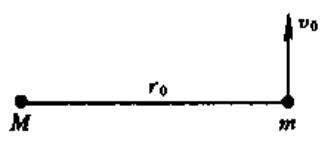
\includegraphics[width=0.25\textwidth]{figures/力图4-3-1.jpg}
\end{center}
\vfill

\textbf{4-4} 空间两质点的质量分别为 $m_{1}$ 和 $m_{2}$，彼此以万有引力相互作用。开始时两质点静止，相距 $r_0$，在引力作用下彼此接近并相碰。试求两质点从开始运动到相碰所经历的时间。
\vfill

\newpage
\textbf{4-5} 如力图4-5-1所示，质量为 $m = 1.20 \times 10^{4}\,\mathrm{kg}$ 的飞船在离月球表面高度为 $h = 100\,\mathrm{km}$ 处绕月球作圆周运动。飞船采用两种登月方式。1. 在 A 点向前（即向力图4-5-1上方）短时间喷气，使飞船与月球相切地到达月球上的 B 点（AB 通过月球中心 O 点）。2. 在 A 点向外侧（即向力图4-5-1右方）沿月球半径短时间喷气，使飞船与月球相切地到达月球上的 C 点（CO 与 AB 垂直）。设喷气相对飞船的速度为 $u = 1.00 \times 10^{4}\,\mathrm{m/s}$。已知月球半径 $R = 1700\,\mathrm{km}$，月球重力加速度（当作常量）$g = 1.700\,\mathrm{m/s^2}$。试求：两种登月方式各需的燃料质量。

\begin{center}
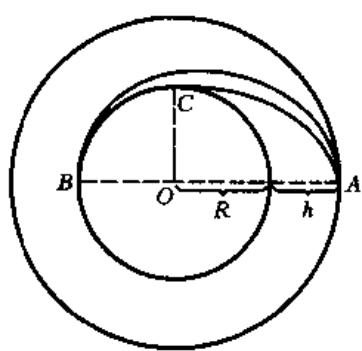
\includegraphics[width=0.2\textwidth]{figures/力图4-5-1.jpg}
\end{center}
\vfill

\textbf{4-6} 如力图4-6-1，飞船绕地球作圆周运动，离地面的高度 $h = 800\,\mathrm{km}$，地球半径 $R = 6.40 \times 10^{3}\,\mathrm{km}$，飞船圆轨道半径 $r_{0} = R + h$，飞船速度 $v_{0} = 3.00 \times 10^{4}\,\mathrm{km/h}$。经过短暂的沿矢径向外侧喷气，飞船获得了指向地心 $O$ 的附加速度 $v_{r} = 800\,\mathrm{km/h}$，其轨道变为椭圆。设喷气后飞船的质量可看作不变。试求：飞船椭圆轨道的近地点和远地点离地面的高度。
\begin{center}
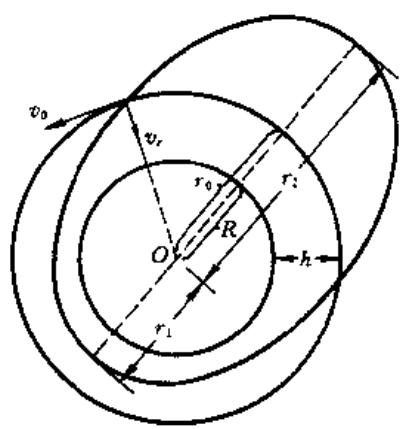
\includegraphics[width=0.2\textwidth]{figures/力图4-6-1.jpg}
\end{center}
\vfill

\newpage
\textbf{4-7} 如力图4-7-1，飞船总质量为 $m$，内装质量为 $m_0$ 的探测器，绕地球沿椭圆轨道运行，近地点与地心距离为 $r_1$，速度为
\[
v_{1} = \sqrt{\frac{2\alpha GM}{r_1}}
\]

1. 试证明 $1 > \alpha > \dfrac{1}{2}$。

2. 如力图4-7-2，飞船在近地点向前发射探测器，并使探测器沿抛物线轨道运动。发射后，飞船沿圆轨道运行。试求：质量比 $\dfrac{m_0}{m}$ 及发射探测器的相对速度 $u$。

3. 如力图4-7-3，若在远地点以上述相对速度 $u$ 发射探测器，试求探测器运行的轨道。

\begin{center}
    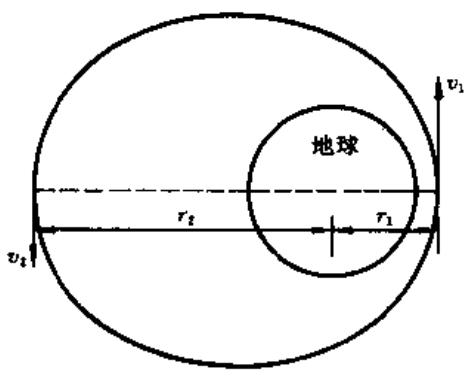
\includegraphics[width=0.16\textwidth]{figures/力图4-7-1.jpg}
    \qquad
    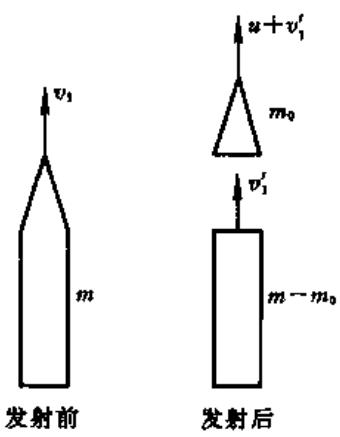
\includegraphics[width=0.16\textwidth]{figures/力图4-7-2.jpg}
    \qquad
    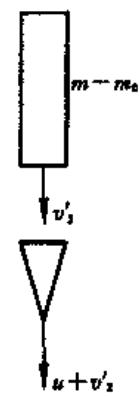
\includegraphics[width=0.08\textwidth]{figures/力图4-7-3.jpg}
\end{center}
\vfill

\textbf{4-8} 如力图4-8-1，地球沿半径为 $R_0$ 的圆轨道绕太阳运动。彗星绕太阳沿抛物线运动。已知抛物线与地球圆轨道一直径的两端相交。忽略地球与彗星之间的引力。

试求：1. 彗星抛物线轨道的方程。2. 彗星的最大速率是地球公转速率的几倍？3. 彗星在地球轨道内的运行时间是多少地球年？
\begin{center}
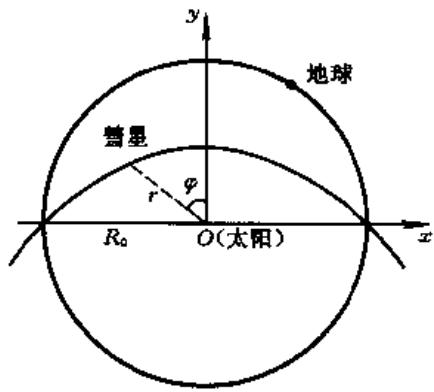
\includegraphics[width=0.2\textwidth]{figures/力图4-8-1.jpg}
\end{center}
\vfill

\newpage
\textbf{4-9} 如力图4-9-1，质量为 $M$ 的宇航站和与其对接上的质量为 $m$ 的飞船一起绕地球沿圆轨道运动，轨道半径是地球半径 $R$ 的 $n$ 倍，$n = 1.25$。某一瞬时，宇航站将飞船沿运动方向发射出去。发射后，飞船和宇航站将分别沿各自新的椭圆轨道运行。已知飞船椭圆轨道的远地点离地球中心的距离为 $8nR$。设发射飞船后宇航站的质量不变（即忽略喷气的质量）。

试问：当质量比 $\dfrac{m}{M}$ 为何值时，飞船绕地球一周后刚好与宇航站相遇。
\begin{center}
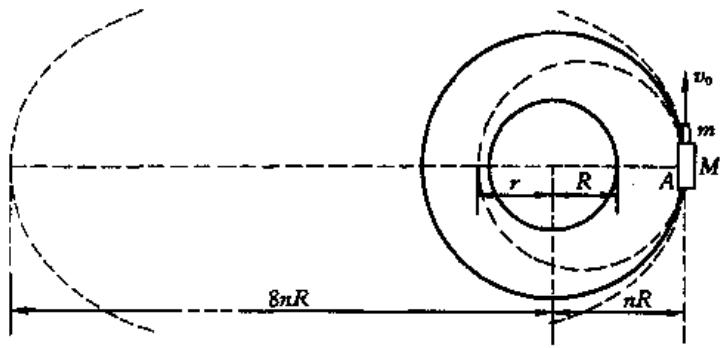
\includegraphics[width=0.3\textwidth]{figures/力图4-9-1.jpg}
\end{center}
\vfill

\textbf{4-10} 如力图4-10-1，从地球发射火箭到火星进行探测，发射后火箭绕太阳沿椭圆轨道运行。为了节省能量，火箭离开地球的速度方向与地球绕太阳公转的速度方向一致，并且选择适当的发射时机，使火箭椭圆轨道的远日点为火星，近日点为地球。假定地球和火星均绕太阳作圆周运动，圆轨道半径分别为 $r_{\text{地}}$ 和 $r_{\text{火}}$，忽略其他行星对火箭的引力作用。

试问：1. 火箭应以多大的相对速度离开地球？2. 火箭到达火星要用多长时间？
\begin{center}
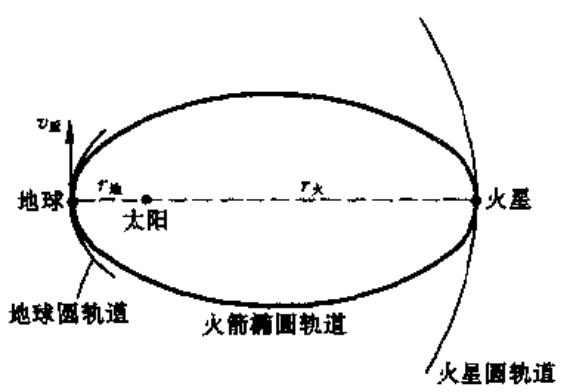
\includegraphics[width=0.3\textwidth]{figures/力图4-10-1.jpg}
\end{center}
\vfill

\newpage
\textbf{4-11} 如力图4-11-1，宇宙飞船绕火星沿圆轨道运行，运动速度为 $v_{0}$。已知火星半径为 $R$，飞船圆轨道离火星表面的高度为 $H$。今飞船在极短时间内，沿圆轨道径向向外侧点火喷气，使飞船获得指向火星的径向速度 $\alpha v_{0}$，$\alpha$ 是远小于1的常数。因喷气量很小，喷气后飞船的质量可视为不变。喷气后，飞船绕火星沿新的椭圆轨道运行。

试求：1. 飞船椭圆轨道近火星点距火星表面的高度 $h_{A}$ 以及远火星点距火星表面的高度 $h_{B}$。2. 飞船绕椭圆轨道的运行周期。
\begin{center}
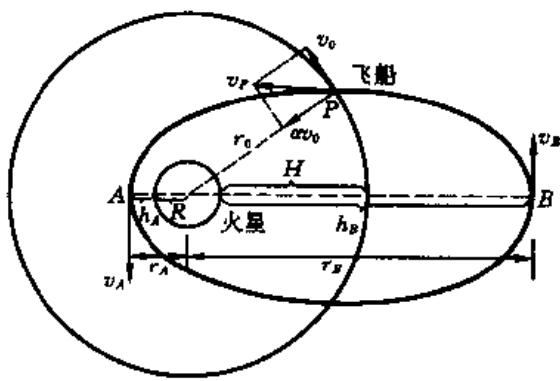
\includegraphics[width=0.3\textwidth]{figures/力图4-11-1.jpg}
\end{center}
\vfill

\newpage

\textbf{4-12} 将宇宙飞船从地面发射到太阳系外，有两个方案。方案一：以足够大的速度（大于太阳系逃逸速度）直接发射。方案二：使宇宙飞船接近太阳系的一个外层行星（例如火星），在它的作用下，改变运动方向，然后逃离太阳系。

试求：1. 按方案一，确定从地面发射飞船所必需的相对地球的最小速度 $v_{a}$ 及发射方向。2. 按本题第1问的方向相对地球以 $v_{b}$ 从地面发射飞船，求飞船穿过火星轨道的速度，即求飞船速度在火星轨道的切线分量和垂直分量。设飞船穿过火星轨道时，火星离飞船很远。3. 使飞船进入火星引力场，但仍可飞出太阳系，求从地面发射的速度。设飞船相对地球的发射方向与本题第一问相同，设飞船沿火星轨道的切线方向脱离火星引力场。4. 估计方案二比方案一节省能量的最大百分比。

设所有行星在同一平面内以同一方向绕太阳在圆轨道上运行。设空气阻力及地球自转的影响均可忽略。

数据：地球绕太阳公转的速度为 $30\,\mathrm{km/s}$，地球到太阳的距离与火星到太阳的距离之比为 $2{:}3$，地球半径 $R_E = 6400\,\mathrm{km}$，地球表面的重力加速度 $g = 9.80\,\mathrm{m/s^2}$。
\vfill

\newpage
\textbf{4-13} 如力图4-13-1，劲度系数 $k = 3$ 的弹簧一端 $O$ 固定，另一端有质量 $m = 20\,\mathrm{g}$ 的质点。质点绕 $O$ 点在光滑水平面内作匀速圆周运动，总机械能为 $E_0 = 12\,\mathrm{J}$。突然沿径向给质点一击，使之获得沿径向向外的速度 $v_{r0} = 1.0\,\mathrm{m/s}$。设弹簧的原长很小，可忽略不计。

1. 试用能量曲线 $(E \sim r)$ 描述质点受打击前、后的运动状态。2. 试求质点运动的半径范围。

\begin{center}
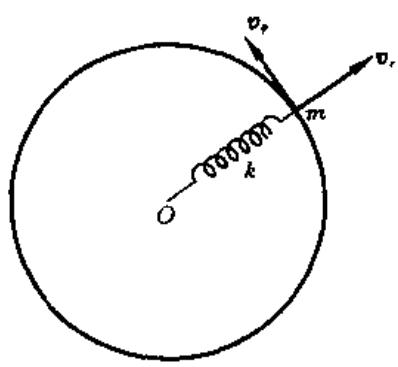
\includegraphics[width=0.2\textwidth]{figures/力图4-13-1.jpg}
\end{center}
\vfill

\textbf{4-14} 一质量为 $m$ 的行星绕质量为 $M$ 的恒星运动。设在行星与恒星之间的整个空间内均匀分布着稀薄的宇宙尘埃，已知尘埃的密度为 $\rho$ 且很小，可以忽略行星与尘埃之间的直接碰撞作用。

1. 试问，对于角动量为 $L$ 的圆形行星轨道，其半径 $r_0$ 应满足什么方程（列出方程即可，不必求解）？

2. 考虑相对上述圆轨道稍有偏离的另一轨道，试解释它是一条作进动的椭圆轨道，进动方向与行星运行方向相反，并求出进动的角速度。
\vfill
